\documentclass[10pt]{beamer}
\usepackage{gensymb} % degree
\usepackage[utf8]{inputenc} %for input tag
\usepackage{siunitx}
\usetheme{metropolis}
\usepackage{appendixnumberbeamer}
\usepackage{amssymb}
\usepackage{xcolor}


\usepackage{booktabs}
\usepackage[scale=2]{ccicons}

\usepackage{pgfplots}
\usepgfplotslibrary{dateplot}

\usepackage{xspace}
\newcommand{\themename}{\textbf{\textsc{metropolis}}\xspace}

\usepackage[export]{adjustbox} %figure
\usepackage{wrapfig}
\usepackage{subfig}
\usepackage{float}
\usepackage{soul}

\usepackage{amsmath}
\usepackage{siunitx}
\usepackage{multimedia}
\usepackage{hyperref}
\usepackage{multicol}

\title{Multi-Robot Task Allocation for logistic applications}
% \subtitle{}

\date{March 21, 2019}
\author{
Davide Zorzi - VR414572	}

\institute{University of Verona}
% \titlegraphic{\hfill\includegraphics[height=1.5cm]{logo.pdf}}
% \begin{figure}
    % \frame{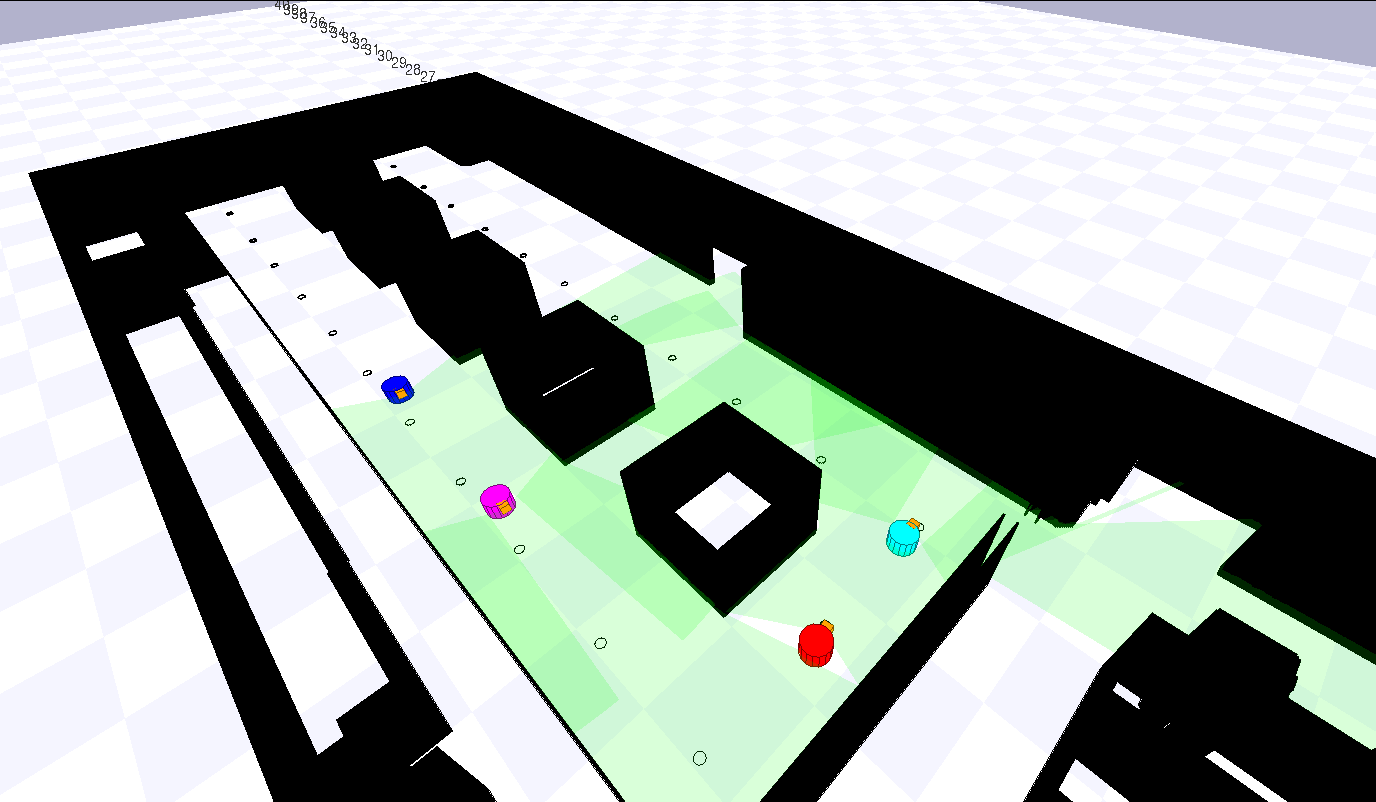
\includegraphics[height= 5cm]{img/prospective.png}}
% \end{figure}

\newcommand{\srst}[0]{SR:ST\space}
\newcommand{\gsp}[0]{GSP1:N\space}
\newcommand{\sps}[0]{SPS1:N\space}
\newcommand{\mrs}[0]{MRS\space}

\begin{document}
	\maketitle
	
	% \begin{frame}{Table of contents}
	% 	\setbeamertemplate{section in toc}[sections numbered]
	% 	\tableofcontents[hideallsubsections]
	% \end{frame}

	
    \begin{frame}[fragile]{Industrial Logistics}
        The {\bf industrial logistics} is the process of {\bf planning}, {\bf organization}
        and {\bf control} of all the activities of handling and {\bf storage} of goods, which, starting
        from the suppliers and reaching up to the end user, guarantee an adequate
        level of {\bf service} to the customer consistent with the {\bf costs} to it associated

        \begin{figure}[hbt]
            \centering
            
\includegraphics[width=\textwidth]{img/ind4.png}
        \end{figure}
    \end{frame}

    \begin{frame}[fragile]{Multi-Robot Systems for logistic applications}

        \begin{figure}[hbt]
            \centering
            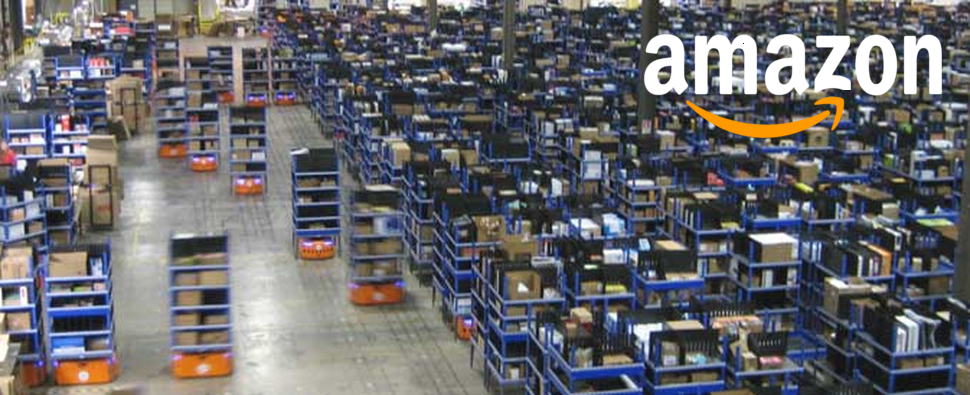
\includegraphics[width=\textwidth]{img/kiva.png}
        \end{figure}
        
        \begin{center}
        Kiva warehouse-management system
        \end{center}
    \end{frame}

    \begin{frame}[fragile]{Thesis contribution}
        \begin{center}
        The contribution of this thesis:
        \end{center}
        \begin{columns}
            \begin{column}{.7\textwidth}
           
            \begin{itemize}
            \item extension of  \texttt{ROS}  package
            \item proposing three tequnique:
            \begin{enumerate}
                \item Single robot : Single task (SR:ST) 
                \item Set Partition Strategy - Single robot : Multiple task (SPS1:N)
                \item Greedy Set Partition Strategy - Single robot : Multiple task (GSP1:N)
            \end{enumerate}
                \item real scenario: Computer Engineering for Industry 4.0 Laboratory (ICE Lab) 
            \end{itemize}
            \end{column}
            \begin{column}{.4\textwidth}
            \begin{figure}
                \subfloat{
\includegraphics[scale=0.45]{img/ros}}\qquad
                \subfloat{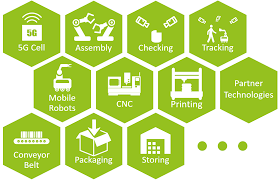
\includegraphics[scale=0.45]{img/ice}}
            \end{figure}
            \end{column}
        \end{columns}
    \end{frame}


    \begin{frame}[fragile]{ICE Laboratory}
        \begin{figure}[hbt]
            \centering
            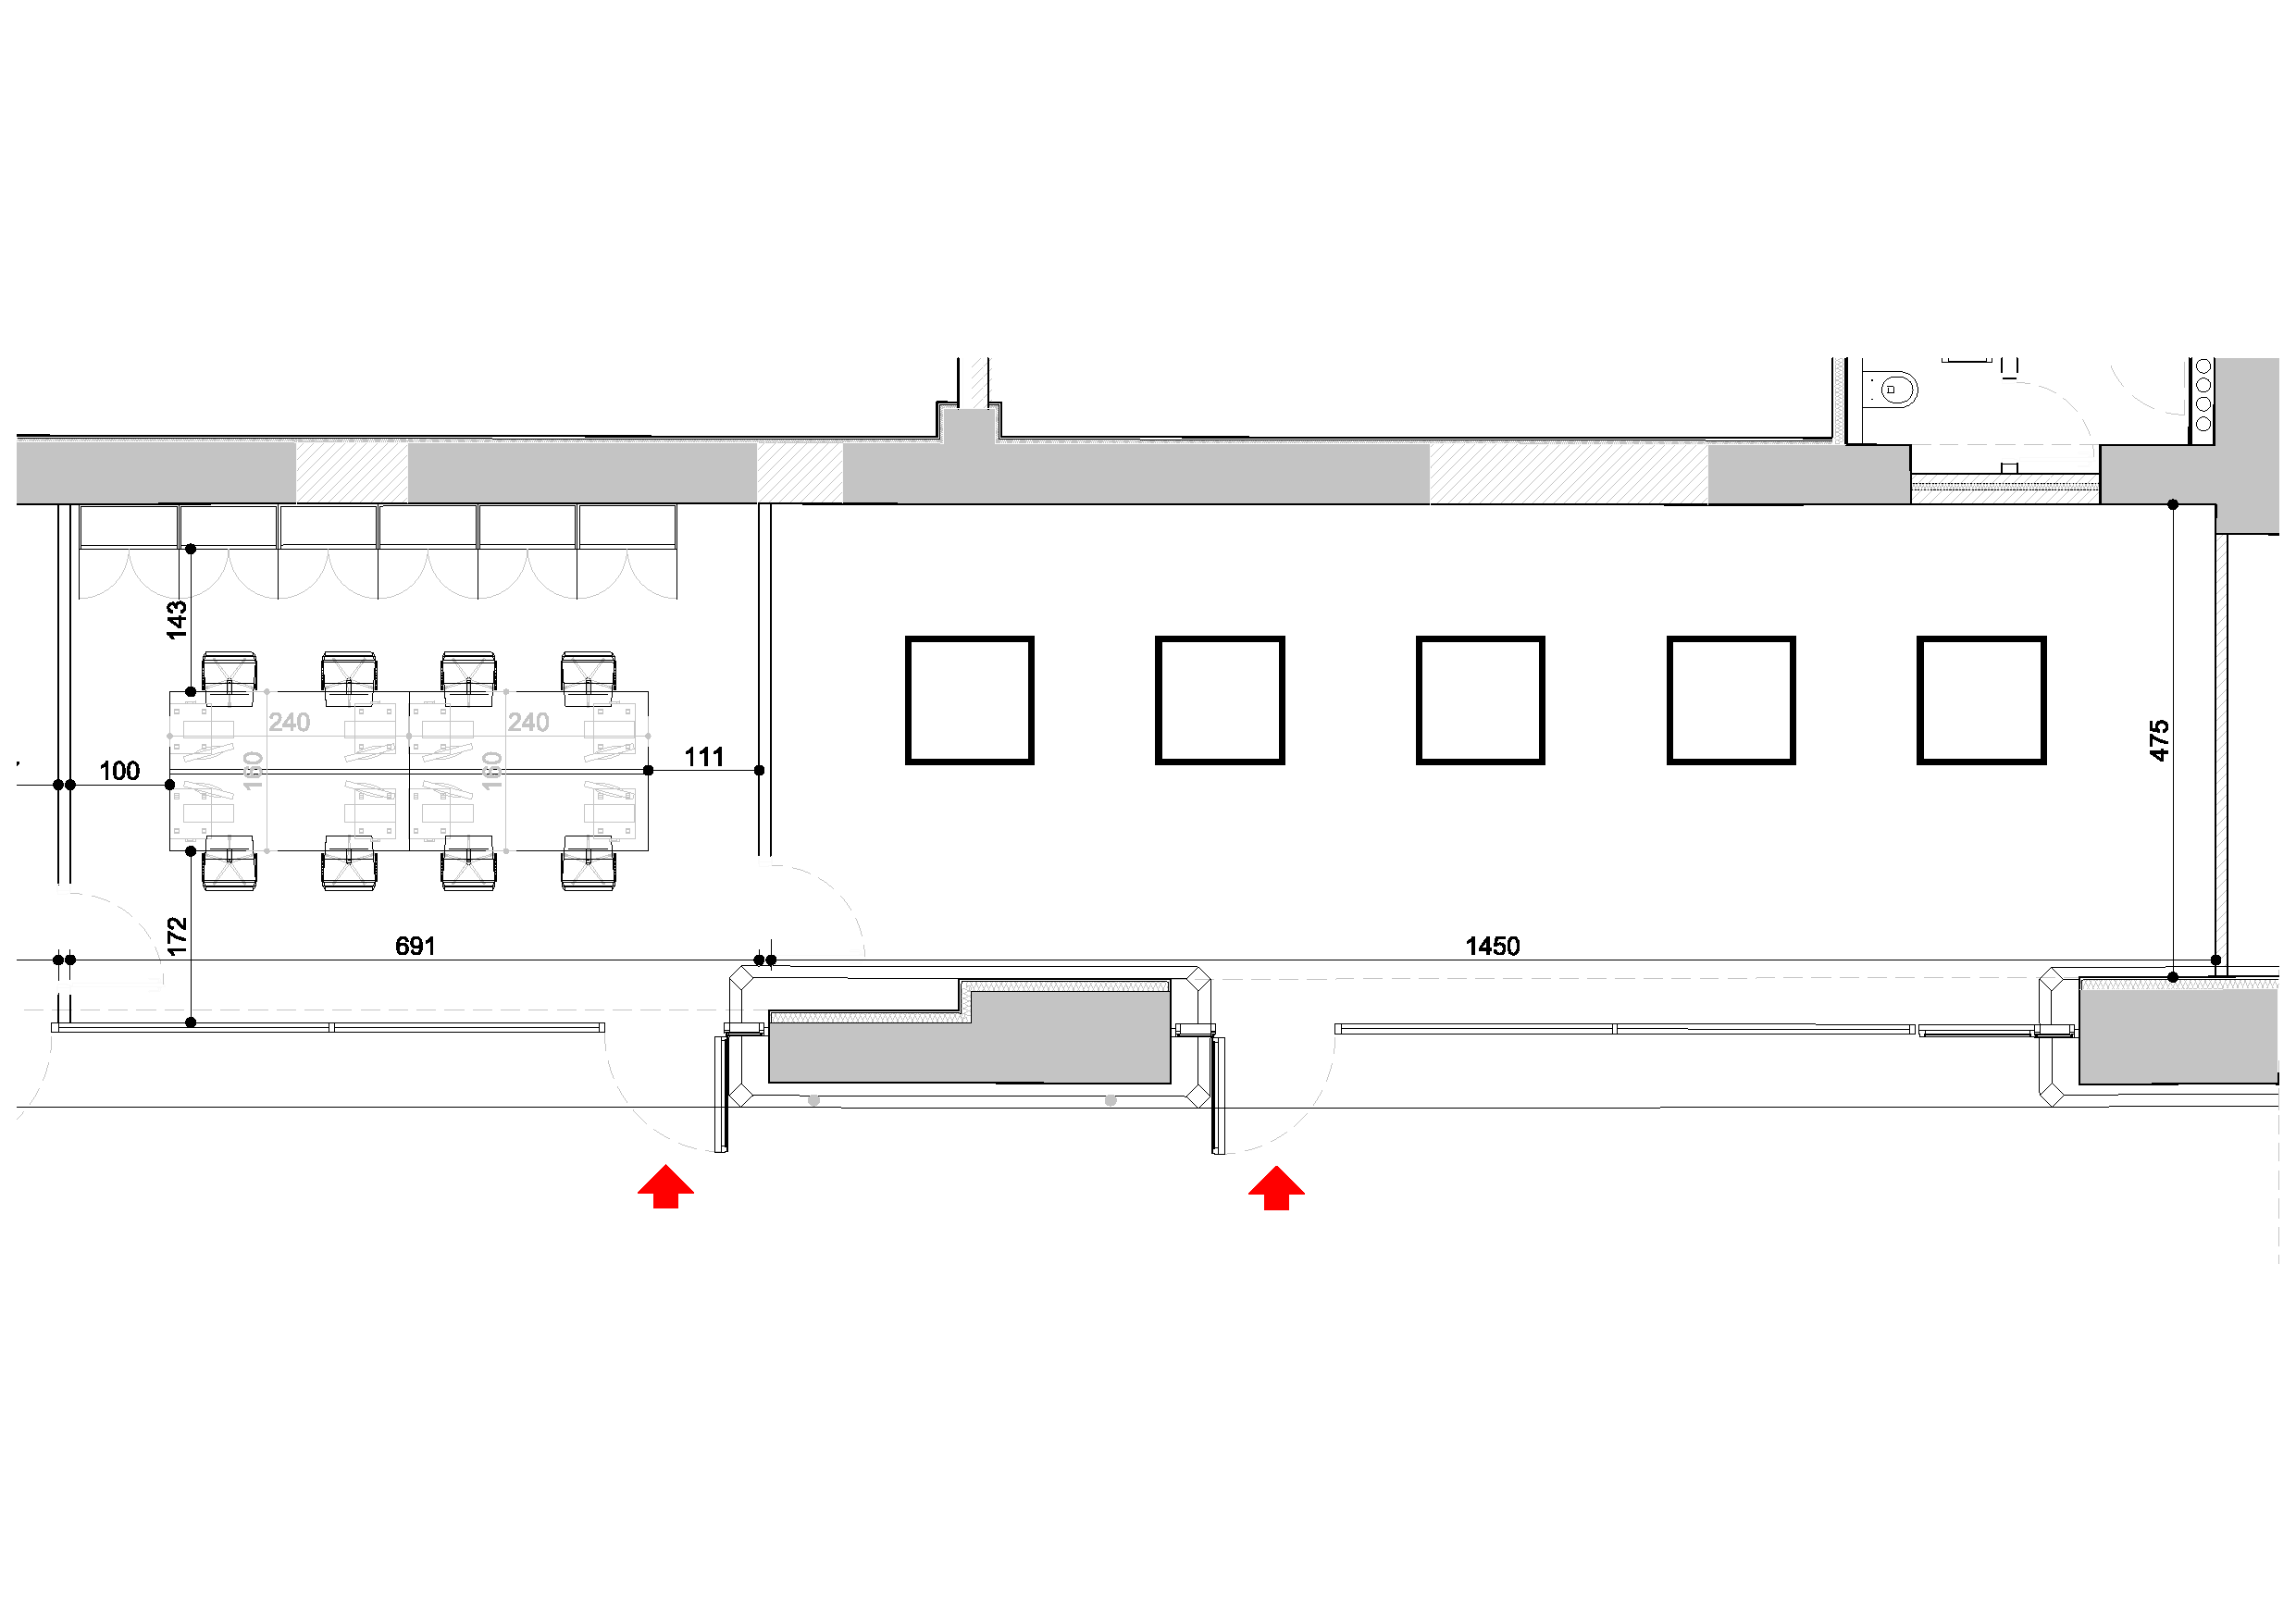
\includegraphics[width=\textwidth]{img/model1}
        \end{figure}
    \end{frame}

    \begin{frame}[fragile]{ICE Laboratory for logistic application}
        \begin{figure}[hbt]
            \centering
            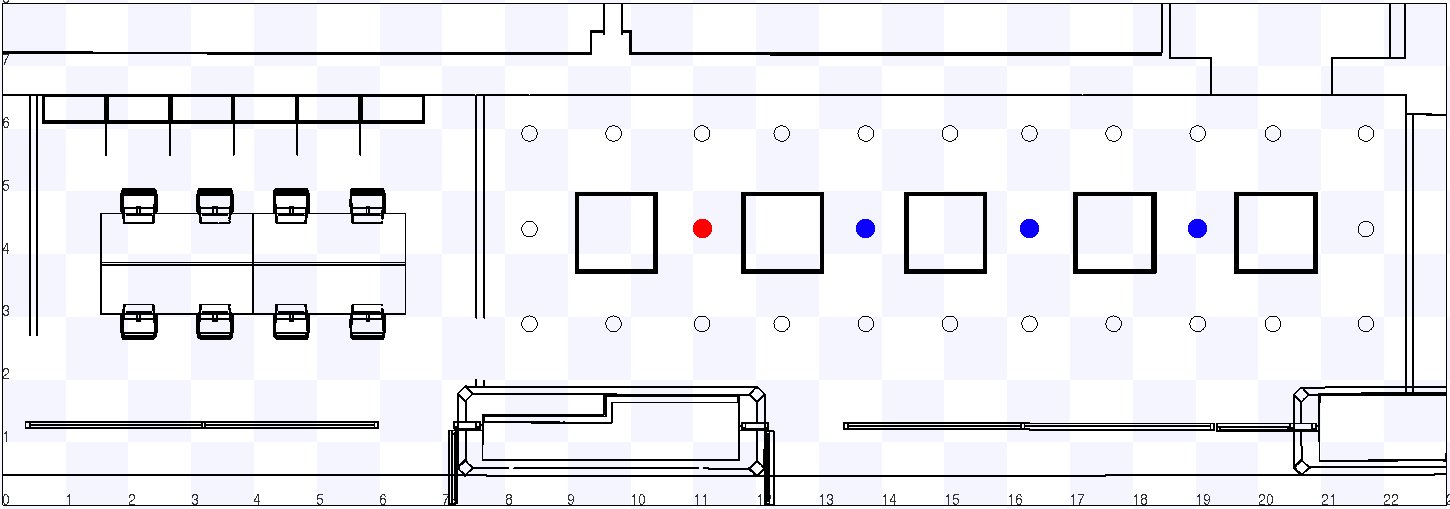
\includegraphics[width=\textwidth]{img/labgrafo}
        \end{figure}

        {\color{red}{$\bullet$}}  Loading bay
        \\
        {\color{blue}{$\bullet$}}  Unloading bays
        \\
        {\color{black}{$\circ$}}  Vertices
    \end{frame}

    \begin{frame}[fragile]{Set Partition Strategy - Single robot : Multiple task (SPS1:N)}
         \begin{columns}
            \begin{column}{.7\textwidth}
                \begin{center}
                    \begin{tabular}{|c|r|c|} \hline
                    \textbf{iteration} & \textbf{partition size} & \textbf{partition} \\ \hline
                    1    & 1    & \{\{a, b, c, d\}\}   \\
                    2    & 2    & \{\{a, b, c\}, \{d\}\}   \\
                    3    & 2    & \{\{a, b, d\}, \{c\}\}   \\
                    4    & 2    & \{\{a, b\}, \{c, d\}\}   \\
                    5    & 3    & \{\{a, b\}, \{c\}, \{d\}\}   \\
                    6    & 2    & \{\{a, c, d\}, \{b\}\}   \\
                    7    & 2    & \{\{a, c\}, \{b, d\}\}   \\
                    8    & 3    & \{\{a, c\}, \{b\},\{d\}\}   \\
                    9    & 2    & \{\{a, d\}, \{b, c\}\}   \\
                    10   & 2    & \{\{a\}, \{b, c, d\}\}   \\
                    11   & 3    & \{\{a\}, \{b, c\}, \{d\}\}   \\
                    12   & 3    & \{\{a, d\}, \{b\}, \{c\}\}   \\
                    13   & 3    & \{\{a\}, \{b, d\}, \{c\}\}   \\
                    14   & 3    & \{\{a\}, \{b\}, \{c, d\}\}   \\
                    15   & 4    & \{\{a\}, \{b\}, \{c\},\{d\}\}   \\ \hline       
                    \end{tabular}
                  \end{center}
            \end{column}
            \begin{column}{.4\textwidth}
            \begin{figure}
                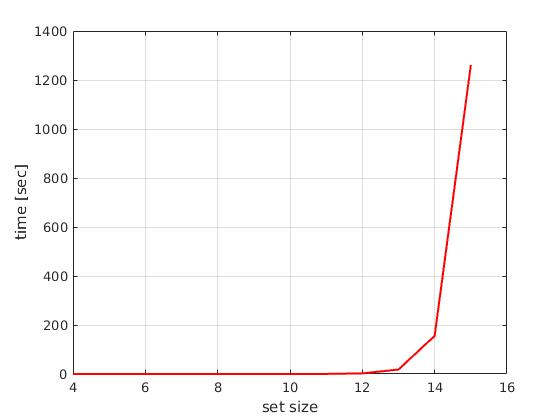
\includegraphics[width=\textwidth]{img/exp}
            \end{figure}
            \end{column}
        \end{columns}
    \end{frame}

    \begin{frame}[fragile]{Greedy Set Partition Strategy - Single robot : Multiple task (GSP1:N)}
    \end{frame}

    \begin{frame}[fragile]{ROS package Logistic\_sim}
        \begin{figure}[hbt]
            \centering
            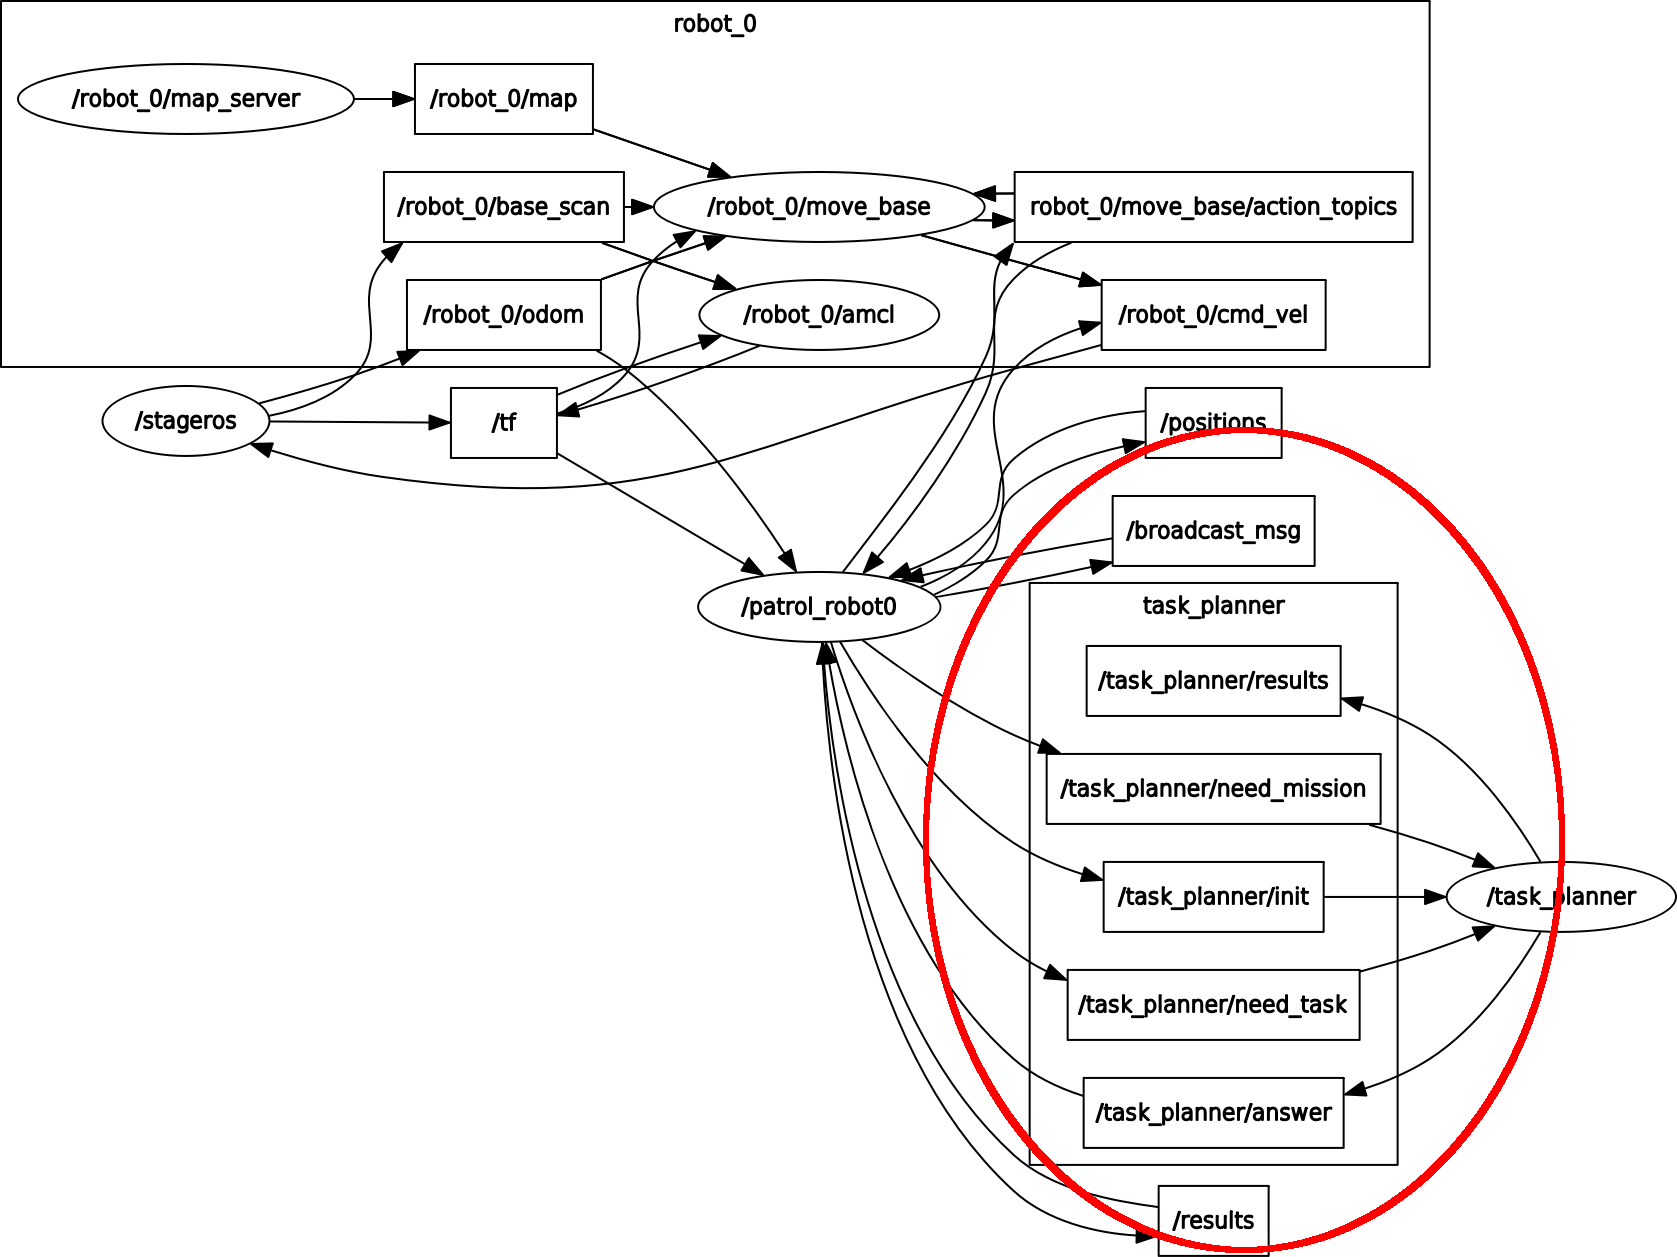
\includegraphics[scale=0.12]{img/rosgraph}
        \end{figure}
    \end{frame}

    \begin{frame}[fragile]{Empirical Results}
    \end{frame}

    \begin{frame}[fragile]{Video}
    \end{frame}

    \begin{frame}[fragile]{Conclusions and Future Work}
    \end{frame}







	
\end{document}